\documentclass[letterpaper,10pt]{article}

\usepackage{titling}
\usepackage{listings}
\usepackage{url}
\usepackage{setspace}
\usepackage{subfig}
\usepackage{sectsty}
\usepackage{pdfpages}
\usepackage{colortbl}
\usepackage{multirow}
\usepackage{multicol}
\usepackage{relsize}
\usepackage{amsmath}
\usepackage{wasysym}
\usepackage{fancyvrb}
\usepackage{amssymb}
\usepackage{ifsym}
\usepackage{amsmath,amssymb,amsthm,graphicx,xspace}
\usepackage[titlenotnumbered,noend,noline]{algorithm2e}
\usepackage[compact]{titlesec}
\usepackage{XCharter}
\usepackage[T1]{fontenc}
\usepackage{tikz}
\usetikzlibrary{arrows,automata,shapes,trees,matrix,chains,scopes,positioning,calc}
\tikzstyle{block} = [rectangle, draw, fill=blue!20, 
    text width=2.5em, text centered, rounded corners, minimum height=2em]
\tikzstyle{bw} = [rectangle, draw, fill=blue!20, 
    text width=4em, text centered, rounded corners, minimum height=2em]

\definecolor{namerow}{cmyk}{.40,.40,.40,.40}
\definecolor{namecol}{cmyk}{.40,.40,.40,.40}

\let\LaTeXtitle\title
\renewcommand{\title}[1]{\LaTeXtitle{\textsf{#1}}}


\newcommand{\handout}[5]{
  \noindent
  \begin{center}
  \framebox{
    \vbox{
      \hbox to 5.78in { {\bf ECE356: Database Systems } \hfill #2 }
      \vspace{4mm}
      \hbox to 5.78in { {\Large \hfill #4  \hfill} }
      \vspace{2mm}
      \hbox to 5.78in { {\em #3 \hfill} }
    }
  }
  \end{center}
  \vspace*{4mm}
}

\newcommand{\lecture}[3]{\handout{#1}{#2}{#3}{Lecture #1}}
\newcommand{\tuple}[1]{\ensuremath{\left\langle #1 \right\rangle}\xspace}

\addtolength{\oddsidemargin}{-1.000in}
\addtolength{\evensidemargin}{-0.500in}
\addtolength{\textwidth}{2.0in}
\addtolength{\topmargin}{-1.000in}
\addtolength{\textheight}{1.75in}
\addtolength{\parskip}{\baselineskip}
\setlength{\parindent}{0in}
\renewcommand{\baselinestretch}{1.5}
\newcommand{\term}{Winter 2018}

\singlespace


\begin{document}

\lecture{ 12 --- File Organization }{\term}{Jeff Zarnett}

\section*{File Organization}

Recall from earlier that there were a few different file organization options we could choose~\cite{fds}:

\begin{enumerate}
	\item \textbf{Heap File}: An unordered file where new records are just appended to the end.
	\item \textbf{Sorted File}: The file is ordered based on a particular field (the sort key).
	\item \textbf{Hashed File}: The file is ordered based on the result of a hash function applied to a particular field.
	\item \textbf{B-Tree File}: The file is organized using a B-tree structure.
\end{enumerate}

We did not go into the details of the options earlier, but we will now be able to do so. Under most circumstances one relation corresponds to one file. However, multiple relations can be in the same file if desired. To start with, we will just have one relation in a file. 

Remember that these file organizations are not affected by whether records are of fixed or variable length. Similarly, whether spanned records is allowed or not does not affect the file organization. Those sorts of consideration are about how to pack records into a block; this is about the order of the records. The first $k$ records may be stored in the first block, but which records are the first $k$?

\subsection*{Heap File} 

The simplest way to order records is: don't order the records! The heap file has no inherent organization, although some (weak) idea of ordering may exist in the sense that records appear in the file in the order in which they are inserted. However, there is no guarantee about that, and if that is the behaviour it is an implementation detail and should not be relied upon. 

This strategy makes insertion efficient -- just tack this on to the end of the file, a constant time ($O(1)$) operation . If a new block is needed, allocate that new block and write it to disk. If not, the last block of the file is read, modified, and written. That part is simple. However, searching for a record is more difficult, because the file is not ordered in any way. Thus, we would have to perform a linear search ($O(n)$) over all records. To find one individual record in the relation it be necessary to examine, on average, half of the entries (assuming that all requests are equally likely). If the element is not in the file at all then we have to examine all the elements, and it was all for nothing anyway~\cite{fds}. 

To delete a record, we need to first search for the record (linear search), then rewrite the block that it is in. Ultimately after enough deletions there will be multiple partially-full blocks, leading to wasted space. Thus, compaction of some sort will eventually need to take place which moves the records around to fill in these holes.

An update has all the problems we've discussed before. We must linear search to find the record(s) to the updated.  it may lead to reorganization of a block or having to move the file to a different block, treating it as if it is an insertion and deletion.  

Heap organization throws into the light the idea that the file structure has performance implications: that is, no matter what we choose, it will mean some operations are faster at the expense of other operations. Heap organization means that insertion is fast but reading, updating, and deleting are slower. This seems incongruous with our usual expectations of what databases are for. Normally we would expect retrieval to be the most common operation, right?

\subsection*{Sorted File}

Long, long ago in an introductory programming course you learned about sorting, and perhaps more importantly, the idea that if you are going to search your data (more than once anyway). Usually in such sorting exercises you are asked to sort a bunch of integers. Integers have nice properties including a logical, simple ordering, and you can tell quickly at a glance if the array has been sorted correctly or not. In a sequential file, we will sort the records based on one particular attribute from start to end.

The field that we sort the file on is called the \textit{ordering field}, and if it is a  unique key then it is called an \textit{ordering key}~\cite{fds}. It does not have to be the primary key. A search that is on the ordering field is quite efficient. Suppose employees have sequential unique employee ID numbers and that is the ordering key in the database. If the goal is to find all employees with an ID less than 385, the data is sequential in all the blocks and that is convenient.

To find an individual record we can use a binary search ($O(\log n)$) which is for finding a record as well as update and deletion as discussed earlier. We are likely to access $\log_{2}(n)$ blocks, whether or not we find what we are looking for.

A simple sequential organization looks like~\cite{dsc}:

\begin{center}
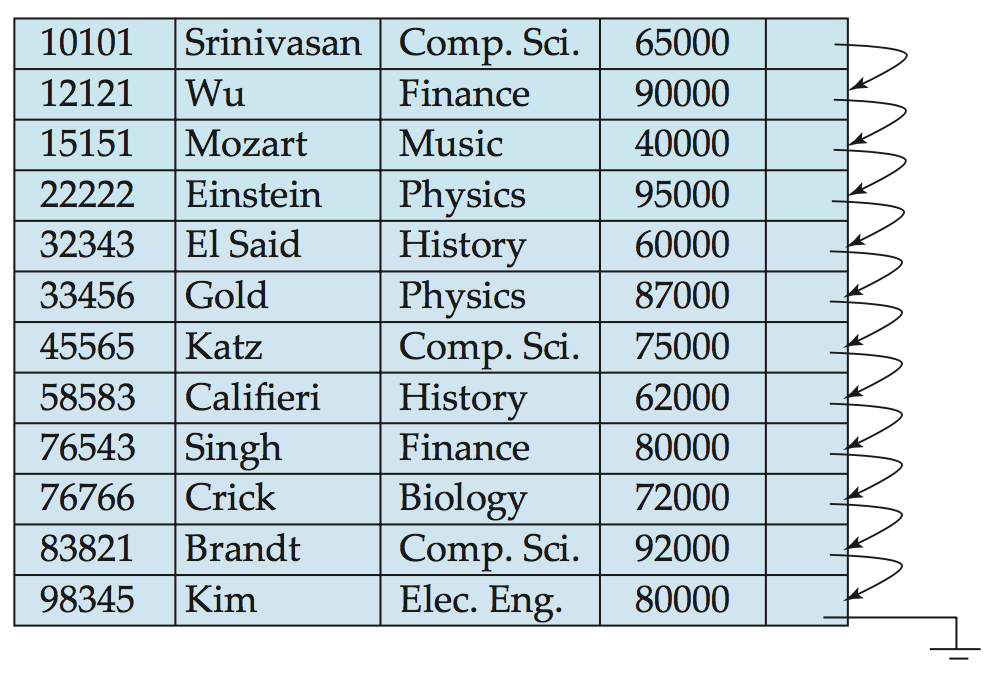
\includegraphics[width=0.4\textwidth]{images/sequential}
\end{center}

In looking at this diagram we can see that they are sorted by some sort of integer ID (the leftmost column) in ascending order. And yet, there is a pointer in the rightmost column pointing to the next record and the next and the next. What purpose would that serve? It is for efficiency reasons, of course. 

It can be difficult to maintain the physical ordering of the data because every insertion, deletion, and perhaps update requires a lot of moving records around. So we could potentially relax the constraint of having to keep all the records in order at all times. Instead, we could temporarily have the following physical layout~\cite{dsc}:

\begin{center}
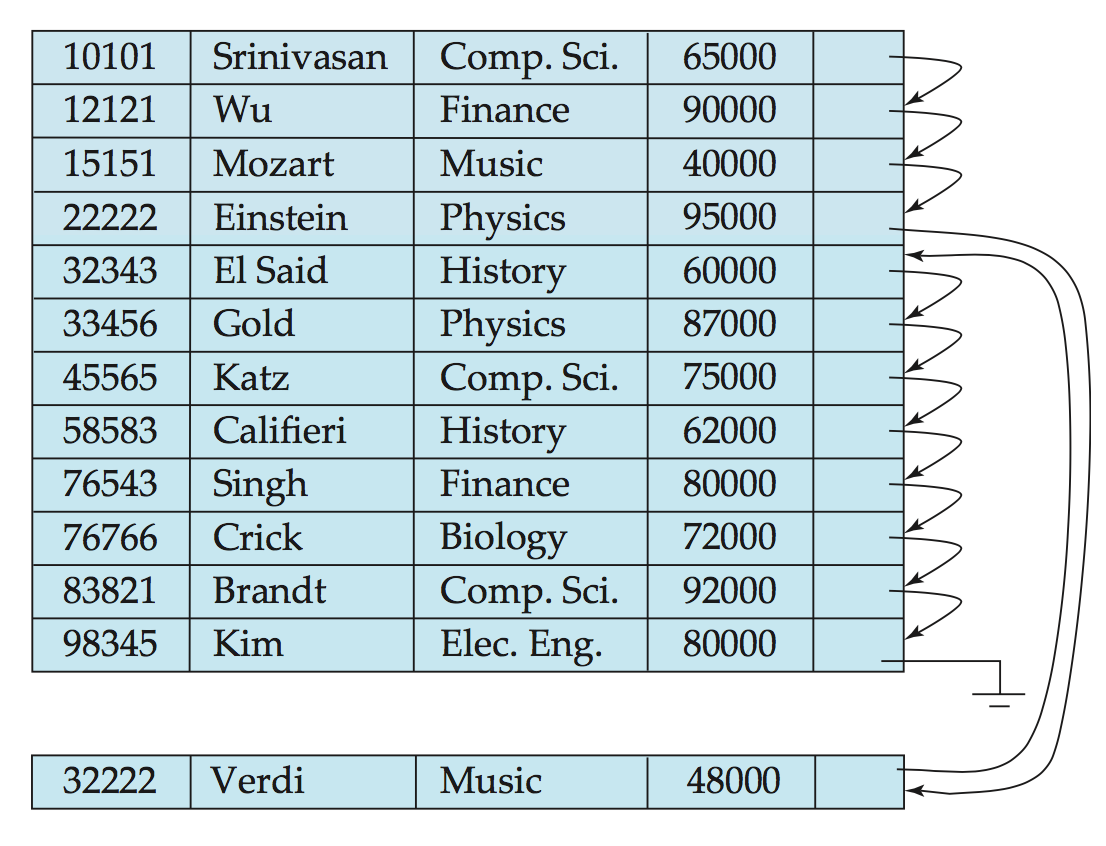
\includegraphics[width=0.45\textwidth]{images/sequential-2}
\end{center}

If the insertion we are doing goes at the end of the file such as in the example an ID of 99001 is inserted, then the file maintains its sequential order. If there is a free space in the block where the record belongs, then we can put the record in the correct block although it is out of order. If, as in the case shown above, the block is full then we need to place the new record somewhere else. For that there is often an \textit{overflow block} where records that do not fit into their normal locations go. 

Deletion is the mirror image of insertion. If we deleted the record at the very end of the file, there is nothing special to maintaining order. If the record being deleted is in an overflow block, that makes the order more sequential rather than less. If the record inside a block is being deleted, such as the record with ID 58583 then the pointer from record 45565 would just be updated to point to 76543 and that would suffice. The empty space would be noted for the future. 

If this continues over time, the file loses its sequential ordering as more and more records end up in overflow blocks. The file becomes less and less sequentially organized, meaning it resembles the heap file more and more. Eventually the file must be reorganized which sorts the records based on the sequential order again, potentially moving a large number of records to get them into the order where they belong. Because this is a potentially expensive operation, it would likely only be done when the system is not busy and when there are enough records out of order that it makes sense to do this. 

\subsection*{Hashed File}

A hashed file works very much like the sorted file, except, instead of the sorting key being a number, a hashed value is used instead. The hash technique can allow for fast access to records. The hash field is often the key. On its own that does not sound any different than the sorted file, but the ``magic'' in the use of the hash function instead of just the ID directly is that the hashed value tells us the address of the disk block in which the record is stored~\cite{fds}. So instead of having to binary search to find the record with ID 99901, we could instead compute the hash value and find out that it is in block $x$ and then go directly there.

We will take a short digression to cover the subject of hashing, actually. Chances are you covered this in a data structures and algorithms course, but it was probably in the context of hashing a value to find what index in the array to insert a particular element. That is \textit{internal hashing}, which we will quickly review, but hashing can be much more.


\bibliographystyle{alphaurl}
\bibliography{356}


\end{document}
